
\documentclass{article} % For LaTeX2e
\usepackage{iclr2026_conference,times}

% Optional math commands from https://github.com/goodfeli/dlbook_notation.
\input{math_commands.tex}

\usepackage{hyperref}
\usepackage{url}

% ------------------------- my packages ----------------
\usepackage{graphicx}  % for including graphics
\usepackage{caption}   % for better caption formatting
\usepackage{float}     % for placement options
\usepackage{booktabs}   % for \toprule, \midrule, \bottomrule, \cmidrule
\usepackage{multirow}   % for multirow/multicolumn cells
\usepackage{caption}    % better caption formatting (optional but recommended)
\usepackage{graphicx}   % if you want to include figures as well
\usepackage{amsmath}    % for math symbols in case of formulas
\usepackage{array}      % for better column formatting

\usepackage{tcolorbox} % Prompt 
\usepackage[T1]{fontenc}
% ---------------------------- -------------------------
% \title{Agentic Retrieval with LLMs for Multi-Hop Question Answering}
\title{PRISM: Agentic Retrieval with LLMs for Multi-Hop Question Answering}
% PRISM (Precision–Recall Iterative Selection Mechanism) 

% Authors must not appear in the submitted version. They should be hidden
% as long as the \iclrfinalcopy macro remains commented out below.
% Non-anonymous submissions will be rejected without review.

\author{Md Mahadi Hasan Nahid \& Davood Rafiei \\
Department of Computing Science\\
University of Alberta, Canada\\
\texttt{\{mnahid, drafiei\}@ualberta.ca} \\
}

% The \author macro works with any number of authors. There are two commands
% used to separate the names and addresses of multiple authors: \And and \AND.
%
% Using \And between authors leaves it to \LaTeX{} to determine where to break
% the lines. Using \AND forces a linebreak at that point. So, if \LaTeX{}
% puts 3 of 4 authors names on the first line, and the last on the second
% line, try using \AND instead of \And before the third author name.

\newcommand{\fix}{\marginpar{FIX}}
\newcommand{\new}{\marginpar{NEW}}

\iclrfinalcopy % Uncomment for camera-ready version, but NOT for submission.


\begin{document}


\maketitle


\begin{abstract}
Retrieval plays a central role in multi-hop question answering (QA), where answering complex questions requires gathering multiple pieces of evidence. We introduce an Agentic Retrieval System that leverages large language models (LLMs) in a structured loop to retrieve relevant evidence with high precision and recall. Our framework consists of three specialized agents: a Question Analyzer that decomposes a multi-hop question into sub-questions, a Selector that identifies the most relevant context for each sub-question (focusing on precision), and an Adder that brings in any missing evidence (focusing on recall). The iterative interaction between Selector and Adder yields a compact yet comprehensive set of supporting passages. In particular, it achieves higher retrieval accuracy while filtering out distracting content, enabling downstream QA models to surpass full-context answer accuracy while relying on significantly less irrelevant information. Experiments on four multi-hop QA benchmarks---HotpotQA, 2WikiMultiHopQA, MuSiQue, and MultiHopRAG---demonstrates that our approach consistently outperforms strong baselines. 

\end{abstract}

% Experiments on four multi-hop QA benchmarks---HotpotQA, 2WikiMultiHopQA, MuSiQue, and MultiHopRAG---demonstrates that our approach consistently outperforms strong baselines. In particular, it achieves higher retrieval accuracy while filtering out distracting content, enabling downstream QA models to achieve answer accuracy on par with using the full context, but with significantly less irrelevant information.

\section{Introduction}

% The problem and challenges
Retrieval systems lie at the heart of question answering, yet designing them remains highly challenging \citep{asai2023selfrag}. Their effectiveness depends on striking the right balance between precision---ensuring that retrieved passages are relevant and free from distracting noise---and recall---guaranteeing that no essential evidence is left behind. This trade-off is especially critical in multi-hop reasoning, where the reasoning chain spans multiple passages: missing even one can break the chain, while excessive irrelevant context can obscure the signal and degrade performance. With the advent of large language models (LLMs), these challenges are amplified. LLMs struggle with the \emph{lost-in-the-middle} phenomenon, overlooking crucial evidence buried in long contexts \citep{liu-etal-2024-lost}, and are prone to hallucination when information is incomplete or noisy \citep{laban-etal-2024-summary}. Thus, enhancing retrieval to provide compact, comprehensive, and faithful evidence is essential for reliable reasoning in LLM-based systems.


These challenges are particularly acute for complex questions requiring multi-hop reasoning, where evidence must be drawn from multiple documents and combined into a coherent chain \citep{yang2018hotpotqa, ho2020constructing, trivedi2022musique}. For example, answering “Which painter who shared a house with Vincent van Gogh was married to a Danish ceramist?” entails finding who shared a house with van Gogh (first hop), then using that result to find who that person married (second hop). Solving such queries is challenging because a system must retrieve the relevant evidence for each reasoning step while ignoring the many distractors present in a large corpus like Wikipedia.

% Existing work and their limitations

% -----
A rich line of research has explored retrieval for multi-hop question answering, yet important gaps remain. Early pipeline approaches such as GraphRetriever and Multi-hop Dense Retrieval \citep{asai2020learning, xiong2021multihop, qi2019answering} relied on iterative query rewriting or entity linking to follow reasoning chains. While effective in controlled settings, these methods suffered from severe error propagation---mistakes in early hops irreversibly degraded final performance. Later frameworks such as ReAct \citep{yao2023react} and IRCoT \citep{trivedi-etal-2023-interleaving} coupled large language models with retrieval, interleaving chain-of-thought \citep{wei2022chain} reasoning and evidence gathering. These approaches improved recall by letting intermediate reasoning guide the search, but often at the cost of large, noisy evidence sets, since precision mechanisms were limited. IRCoT in particular emphasizes recall, leading to distractor-heavy contexts that can obscure reasoning.  

Complementary efforts have aimed to improve relevance and coverage through reranking, as in RankZephyr \citep{pradeep2023rankzephyr}. Likewise, set-wise selection \citep{lee-etal-2025-shifting} suggests that moving beyond naive top-$k$ retrieval---by incorporating reasoning, selection, and refinement---is crucial for complex reasoning. However, these single-pass strategies are limited in that if essential evidence is absent from the initial retrieval pool, there is no mechanism for recovering it. Pruning-based methods such as Provence \citep{chirkova2025provence} improve efficiency by discarding irrelevant passages, but risk harming recall when essential evidence is mistakenly removed. Iterative self-refinement methods (e.g., Self-RAG \citep{asai2023selfrag}) attempt to balance these trade-offs, but lack a principled way to separate precision from recall, often generating redundant or hallucinated context.  

%At a broader level, work has identified inherent limitations in embedding-based retrieval itself. 
%Recent work has highlighted that single-vector embedding retrieval is not just data- or training-limited, but structurally constrained. \citet{weller2025theoreticallimitationsembeddingbasedretrieval} show that fixed-dimensional embeddings cannot, in principle, represent all possible query-document relevance patterns when the space of potential top-k combinations grows combinatorially. Long-context LLM studies further underscore this challenge. \citet{liu-etal-2024-lost} show that models systematically overlook information buried in the middle of extended contexts (``lost in the middle''), while \citet{laban-etal-2024-summary} highlight how irrelevant material in long contexts increases hallucination which can be crucial for complex question answering task. Together, these findings emphasize that simply scaling context or embeddings cannot resolve the precision--recall dilemma. 
% -----

% On the Theoretical Limitations of Embedding-Based Retrieval --> https://arxiv.org/pdf/2508.21038 

%However, a key challenge remains: selecting an optimal set of evidence that is both comprehensive and concise. Standard retrievers or rerankers focus on relevance scoring, which may yield a top-$k$ list that is individually relevant but collectively redundant or incomplete. Prior work has begun to address this by selecting passages as a set rather than ranking them. These trends suggest that moving beyond naive top-$k$ retrieval—by incorporating reasoning, selection, and refinement—is crucial for multi-hop QA

Despite these advances, a key challenge remains: constructing evidence sets that are both \emph{comprehensive and concise}. Standard retrievers and rerankers typically return a top-$k$ list of individually relevant passages, but the set as a whole is often redundant or incomplete. More broadly, retrieval-augmented generation faces fundamental limitations: (i) single-vector embeddings cannot represent all possible query–document relevance patterns as candidate sets grow combinatorially \citep{weller2025theoreticallimitationsembeddingbasedretrieval}; (ii) long-context LLMs systematically overlook mid-context evidence \citep{liu-etal-2024-lost}; and (iii) irrelevant material in long contexts increases hallucination \citep{laban-etal-2024-summary}. Together, these findings highlight that simply scaling embeddings or extending context windows cannot resolve the precision–recall trade-off.

In this work, we introduce \textbf{PRISM} 
(Precision–Recall Iterative Selection Mechanism), an agentic retrieval framework that explicitly separates precision-oriented filtering from recall-oriented addition in an iterative loop. Concretely, PRISM employs three collaborating agents: a \textbf{Question Analyzer} that decomposes the question into sub-questions targetting the required facts; a \textbf{Selector} that filters the candidate pool to eliminate distractors; and an \textbf{Adder} that reconsiders unselected candidates to recover any overlooked evidence. The Selector and Adder iterate, refining the evidence set until it is both compact and complete.

Our contributions are threefold. \textbf{(1)} We propose \textbf{PRISM}, an agentic retrieval framework that explicitly separates precision-oriented filtering from recall-oriented addition, enabling fine-grained control over the precision–recall trade-off in multi-hop QA. \textbf{(2)} We show that PRISM consistently produces evidence sets that are both compact and complete, achieving higher precision and recall than recent baselines on HotpotQA, 2WikiMultiHopQA, MuSiQue, and MultiHopRAG. \textbf{(3)} We demonstrate that these improved evidence sets translate into stronger end-to-end QA, allowing LLM readers to match or surpass full-context performance, with notable gains on the most challenging multi-hop benchmarks where distractors typically hinder accuracy.

% ------------- --------------


\begin{figure}[t] % [t] = place at top of page; you can also use [h] or [b]
    \centering
    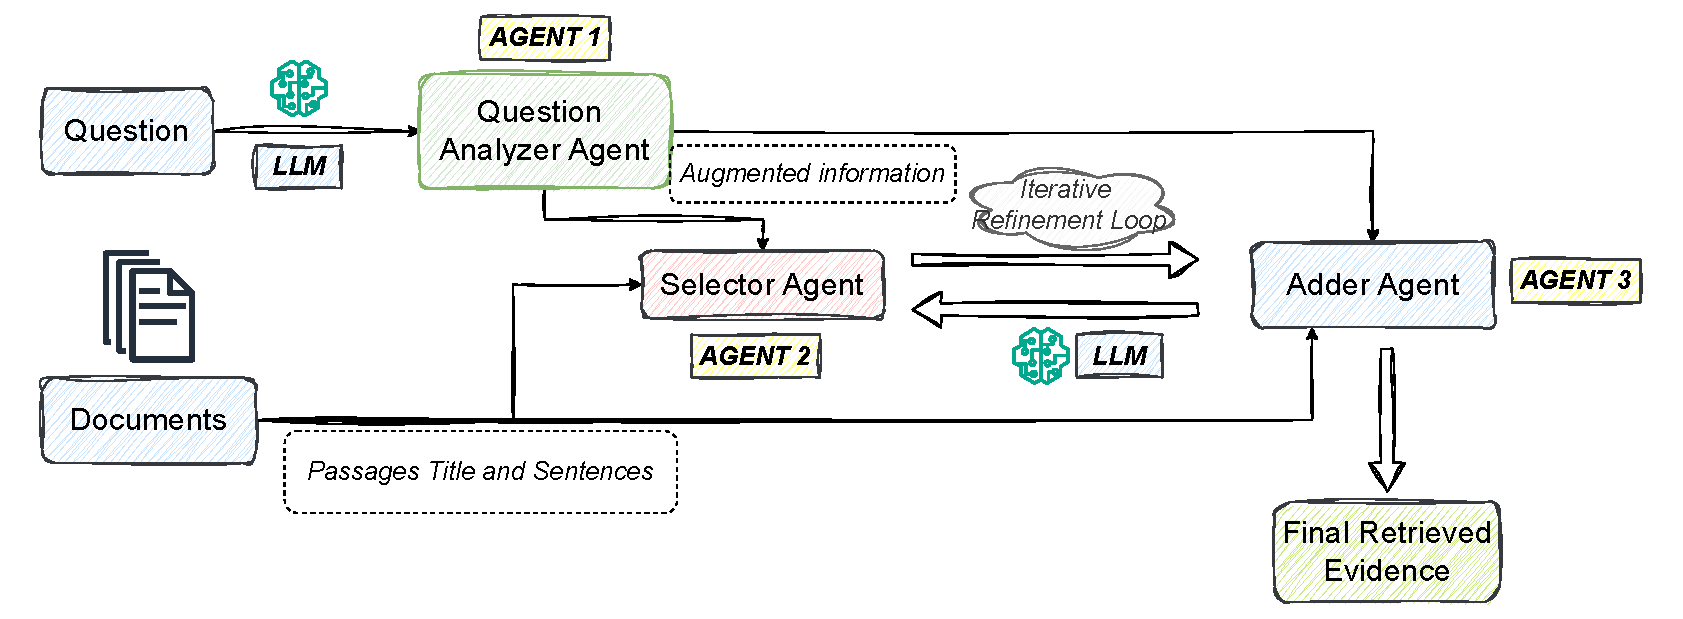
\includegraphics[width=1.0\linewidth]{figures/ir-agent-sketch-2-2.pdf}
    \caption{Overview of Agentic Retrieval Framework (PRISM). The complex question is decomposed by the Analyzer into sub-questions, the Selector narrows down relevant evidence for precision, and the Adder expands context for recall. The loop iterates $N$ times to produce a refined evidence set for QA.}
    \label{fig:framework_overview}
    \vspace{-0.8em}
\end{figure}


\section{Methodology}
\label{sec:methodology}

% Overview of the Agentic Retrieval System

We propose \textbf{PRISM} (Precision–Recall Iterative Selection Mechanism), 
an agentic retrieval framework that decomposes the multi-hop evidence gathering process 
into a sequence of coordinated steps. PRISM employs three LLM-based agents with distinct roles: the \textbf{Question Analyzer}, which decomposes complex queries into sub-questions; the \textbf{Selector}, which filters candidate evidence to maximize precision; and the \textbf{Adder}, which supplements missing evidence to improve recall. 
Each agent is instantiated as a prompted LLM with instructions tailored to its task. Operating in an iterative loop, these agents collectively produce a compact yet comprehensive set of supporting passages. Figure~\ref{fig:framework_overview} illustrates the overall architecture and data flow. We provide an illustrative example in the Appendix \ref{app:illustrative_example}.

\subsection{Question Analyzer Agent}

Multi-hop questions often intertwine multiple entities, relations, and constraints into a single complex query, making it easy for retrievers or LLMs to chase partial matches or irrelevant context. The Question Analyzer mitigates this risk by decomposing the query into a structured set of sub-questions that make the evidence requirements explicit and define a focused search space for later agents \citep{fu-etal-2021-decomposing-complex}. This decomposition reduces the chance of missing critical hops while preventing downstream stages from being overwhelmed with loosely relevant candidates. Concretely, we prompt an LLM with a decomposition template that encourages explicit reasoning, and it returns a list of sub-questions, each targeting a distinct factual unit required to answer the original query.
%The role of the Question Analyzer is to understand the multi-hop question and split it into manageable parts. We prompt the LLM with a template that encourages explicit decomposition. Multi-hop questions often bundle several entities, relations, and constraints into one complex query; without decomposition, retrievers and LLMs risk chasing partial matches or irrelevant context. By breaking the question into sub-questions, the Analyzer makes the evidence requirements explicit and defines a structured search space. This step not only lowers the likelihood of missing critical hops but also prevents later agents from being overloaded with loosely relevant candidates. In effect, the Analyzer acts as the scaffolding that guides the precision and recall stages toward the right evidence.
%The agent leverages the LLM’s inner knowledge and language understanding to perform this analyzing task. We provide LLM with the detail instruction to understand and decompose the complex multi-hop question and take response as a list of subquestions.  


\subsection{Selector Agent}

The Selector serves as a precision-focused filter that removes distractors introduced during retrieval. Large corpora inevitably yield passages that share surface-level words with the query but are semantically off-topic, and passing such noise directly to a QA model leads to error propagation and wasted context budget. The Selector mitigates this by enforcing a high bar for inclusion: it anchors the reasoning chain with the relevant passages that are strongly aligned with the sub-questions. %This explicit precision stage prevents hallucinations and reduces lost-in-the-middle effects, ensuring that downstream reasoning starts from reliable, compact evidence. 

Concretely, the agent is prompted with detailed instructions, the sub-questions, and the retrieved  passages, and tasked with  outputting only those that directly support the query. This filtering stage yields evidence sets with very high precision, ensuring that downstream reasoning operates over reliable, compact inputs and mitigating hallucinations as well as lost-in-the-middle effects. The trade-off, however, is that some relevant passages may be excluded if their connection is less explicit—a limitation addressed by the Adder agent in the next stage.

%The effect of the Selector is to remove noise to improve precision. For instance, a BM25 retrieval might return some passages that share keywords with the sub-question but are contextually irrelevant. The LLM, with its deeper understanding of semantics, often can judge that those passages do not actually pertain to the question. This leads to a very high precision in the selected set – typically, nearly every passage chosen by the Selector is genuinely a supporting fact. Of course, the trade-off is that the LLM might miss a relevant passage if it’s not obviously connected or if it appears less related at first glance. That is why we introduce the Adder agent next.


\subsection{Adder Agent}
While precision is vital, overly strict filtering risks omitting complementary or bridging facts that are crucial for multi-hop reasoning. The Adder is introduced to counterbalance this risk by explicitly prioritizing recall. Its role is to audit what the Selector left behind and add evidence that fill logical gaps—such as a spouse relation that pairs with a shared-house relation, or a bridging entity connecting two documents. This two-phase design, ensures that the final evidence set is both compact and complete. The instructions for the Adder agent are similar to the Selector’s, but with a different emphasis. We provide it with the same list of candidates, the sub-questions, and additionally indicate which evidence have already been selected by the Selector. 

In essence, the Adder is a second pass through the candidates, but primed to look for anything important that was left out. One common scenario is when the answer to the sub-question actually requires combining two facts from different passages. The Selector might pick one of them (e.g. a passage that gives part of the answer), not realizing another evidence from different passage is also needed for the full answer. The Adder, seeing what’s selected and what the question is, can identify the complementary piece. In the ideal outcome, after the Adder, the union of selected + added passages equals the complete set of supporting documents needed for answering the question. If the Selector already did a perfect job, the Adder will simply output nothing new. But if something was missing, the Adder ensures recall goes up. This two-phase selection is analogous to having a strict filter followed by a gentle filter: one says “only keep absolutely sure things”, the next says “don’t leave out anything that might be required”.

\subsection{Iteration and Multi-Hop Handling}
Multi-hop questions typically require reasoning over multiple intermediate facts. After decomposition by the Question Analyzer, we provide the original question and all generated sub-questions together to the Selector and Adder agents. This joint formulation allows the Selector$\Leftrightarrow$Adder Cycle to identify the minimal set of evidence that collectively cover the reasoning chain.  

The Selector$\Leftrightarrow$Adder cycle is repeated for several iterations, with the evidence set refined at each step. At the end of the process, evidences from all iterations are merged and de-duplicated, producing a compact set that typically contains only the essential evidence required for the multi-hop question while maintaining high precision and recall. This final set is then passed to a  Answer Generator agent. 

\subsection{Answer Generator Agent}
To demonstrate the overall question answering performance of our retrieval framework we introduce a \textbf{Answer Generator} agent, which produces the answer given the retrieved evidence set using our proposed framework. After the Question Analyzer, Selector, and Adder agents collaboratively construct a compact but comprehensive set of supporting evidence, we provide this context along with the original question to a large language model instructed to generate the final answer. We implement the Answer Generator as a prompted LLM operating in a \textbf{zero-shot} setting, without task-specific fine-tuning. 
This design choice allows us to directly assess how improvements in retrieval quality translate into downstream QA performance, while avoiding additional supervision or domain adaptation. 


\section{Experimental Setup}

\subsection{Datasets}
We evaluate our framework on three standard multi-hop QA benchmarks in the open-domain setting, where supporting passage and/or facts can be retrieved from a corpus, and additionally include the MultiHop-RAG \citep{tang2024multihoprag} dataset for specialized retrieval analysis. \textbf{HotpotQA} \citep{yang2018hotpotqa} contains questions requiring reasoning over multiple paragraphs, and we use its open-domain variant in which systems must retrieve relevant paragraphs from the full Wikipedia index, with supporting sentences provided for evaluation. \textbf{2WikiMultiHopQA} \citep{ho2020constructing} features questions that connect two Wikipedia pages via shared entities; following prior work, we employ only the structured text component using its development set. \textbf{MuSiQue} \citep{trivedi2022musique} consists of questions requiring 2–4 reasoning hops and was specifically constructed to prevent reasoning shortcuts; we use the answerable subset defined by \citet{trivedi-etal-2023-interleaving}. \textbf{MultiHop-RAG} \citep{tang2024multihoprag}, a recently proposed benchmark in the RAG (Retrieval-Augmented Generation) domain, introduces multi-hop queries over a news-article knowledge base; we use this dataset particularly to assess the retrieval precision and recall of evidence selection in our framework. \footnote{For evaluation, we sample 500 instances from each dataset, constrained by computational budget, while ensuring that the subset remains representative of the overall distribution. }

\subsection{Baselines and Evaluation Metrics}
\paragraph{Baselines.}
We compare our Agentic Retrieval framework against several strong baselines. \textbf{IRCoT} \citep{trivedi-etal-2023-interleaving} couples chain-of-thought reasoning with iterative retrieval. \textbf{SetR} \citep{lee-etal-2025-shifting} performs set-wise reranking with LLM reasoning, which we approximate by instracting LLMs to select a subset from the top-20 retrieved passages in a single step. \textbf{Oracle Gold} uses gold supporting paragraphs provided by the datasets, representing an upper bound for retrieval and QA. We also report a \textbf{No Retrieval (Full Context)} baseline, where LLMs answer questions using full context, and compare our results against DSP  \citep{khattab2022demonstrate}, DecomP  \citep{khotdecomposed}, RankZephyr  \citep{pradeep2023rankzephyr}, and RankGPT  \citep{sun-etal-2023-chatgpt}. 

\paragraph{Evaluation Metrics.}
We assess retrieval using standard supporting fact metrics, treating each passage as the retrieval unit. A passage is correct if it contains at least one gold supporting sentence (HotpotQA, 2WikiMultihopQA) or matches a labeled supporting paragraph (MuSiQue, MultiHopRAG). We report \textbf{Precision} (fraction of retrieved passages that are gold) and \textbf{Recall} (fraction of gold passages retrieved), and also track 
the number of retrieved passages, as compact evidence sets improve efficiency and reduce noise. For HotpotQA and 2WikiMultihopQA, we additionally report \textbf{fact-wise precision and recall} at the sentence level. End-to-end QA is evaluated with \textbf{Exact Match (EM)} and token-level \textbf{F1}. We further measure performance under three conditions: (i) \textit{full context}, where the QA model sees all 
retrieved passages including distractors, (ii) \textit{retrieved evidence only}, using the filtered set from our framework, and (iii) \textit{gold evidence only}, where the QA agent receives only the labeled supporting facts. This setup enables us to evaluate both retrieval quality and its effect on QA accuracy.

\subsection{Implementation Details}
\label{sec:llms}

We implement all agents as prompted large language models. Unless stated otherwise, we use {GPT-4o} \citep{OpenAI_gpt4o_system_card_2024}, {Gemini-2.0-Flash-Lite}\citep{google_gemini2.5_report_2025} and {DeepSeek-Chat}\citep{deepseek_ai_deepseek-v3_2024}, all state-of-the-art models with large context windows, enabling evaluation over all candidate passages. Prompting is performed in a zero-shot setting, without task-specific fine-tuning. We enforce consistent structured outputs (lists of indices/titles) to ensure reliable parsing. The Selector$\Leftrightarrow$Adder cycle is repeated at most $N=3$ iterations, keeping the number of LLM calls tractable. As shown in Section~\ref{sec:results}, the system achieves strong retrieval performance, which directly translates into higher Question Answering accuracy.  


\section{Results and Discussion}
\label{sec:results}
\subsection{Main Result}

% \begin{figure}[ht]
%     \centering
%     
\includegraphics[width=0.9\linewidth]{iclr2026/figures/recall_no_gaps-2.pdf}
%     \caption{Passage recall across HotpotQA, 2WikiMultihopQA, and MuSiQue. 
% Our agentic retrieval framework consistently outperforms OneR and IRCoT  \citep{trivedi2023ircot}, achieving state-of-the-art recall on all three datasets. 
% The gains are especially notable on the challenging MuSiQue benchmark, 
% demonstrating the effectiveness of combining precision-oriented selection with recall-oriented addition in an iterative agentic loop.}
%     \label{fig:recall}
% \end{figure}

\begin{figure}[ht]
    \centering
    \vspace{-0.6em}
    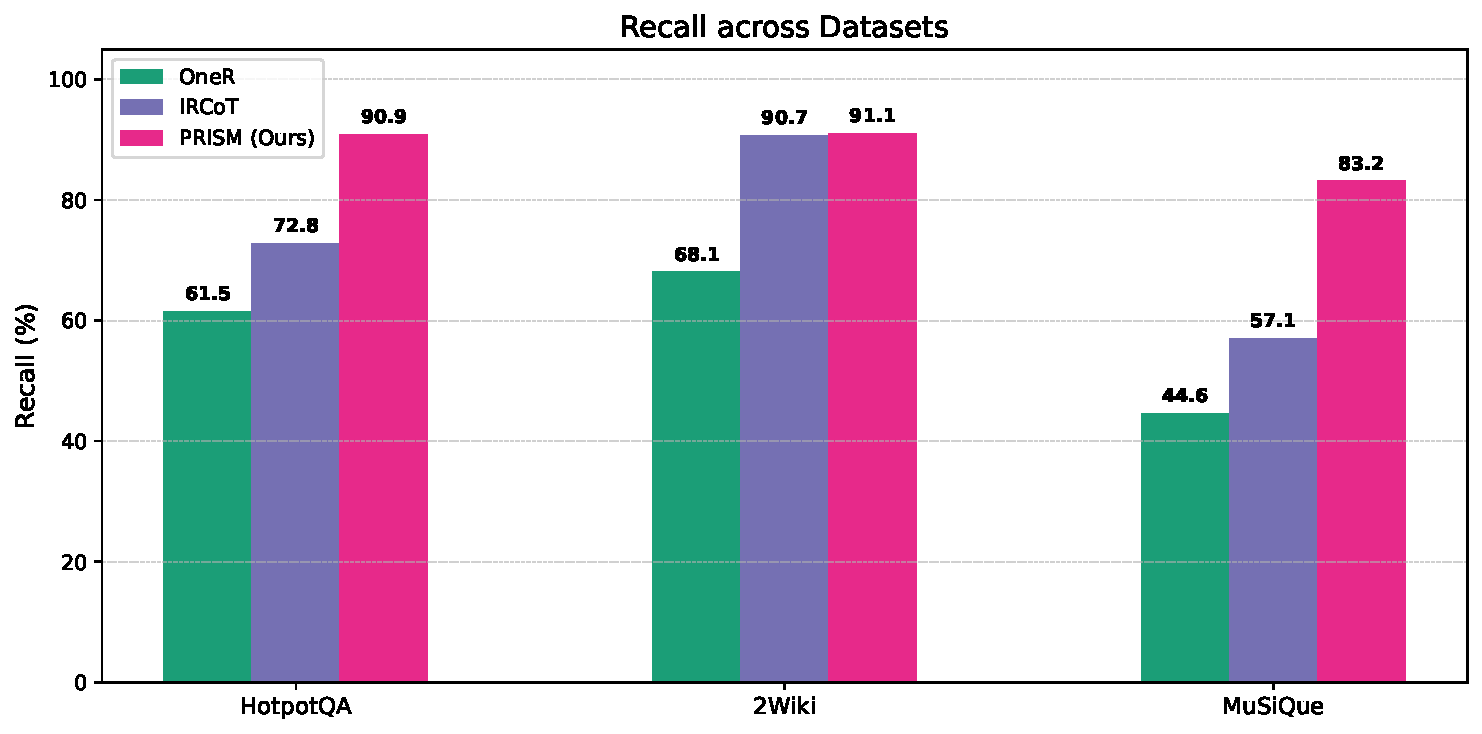
\includegraphics[width=0.8\linewidth]{figures/recall_no_gaps-2.pdf}
    \vspace{-0.8em}
    \caption{ Passage recall across HotpotQA, 2WikiMultiHopQA, and MuSiQue. 
Our agentic retrieval framework (PRISM) consistently outperforms OneR and IRCoT \citep{trivedi2023ircot}, 
with especially large gains on the challenging MuSiQue benchmark.}
    \label{fig:recall}
    \vspace{-0.6em}
\end{figure}

\paragraph{Retrieval Performance.}

Figure~\ref{fig:recall} reports recall performance across HotpotQA, 2WikiMultihopQA, and MuSiQue dataset. Our agentic retrieval framework achieves consistently higher recall than both OneR (one pass retriever), which utilize BM25 \citep{robertson2009probabilistic} to retrieves $K$ paragraphs using the original question as a single query, and IRCoT, which guides retrieval through Chain-of-Thought reasoning, across all benchmarks  \citep{trivedi2023ircot}. On HotpotQA, our method attains \textbf{90.9\%} recall compared to 61.5\% for OneR and 72.8\% for IRCoT. On 2WikiMultihopQA, we reach \textbf{91.1\%} recall, improving over OneR (68.1\%) and slightly exceeding IRCoT (90.7\%).  The largest margin appears on MuSiQue, where our approach achieves \textbf{83.2\%} recall versus 44.6\% and 57.1\% for OneR and IRCoT, respectively. 
These gains validate the importance of explicitly balancing precision and recall through our Selector$\Leftrightarrow$Adder loop: the Selector removes distractors while the Adder recovers missed but necessary passages, ensuring a comprehensive evidence set. 
% The strong improvements, especially on the challenging MuSiQue dataset, demonstrate that our framework generalizes well across diverse multi-hop reasoning scenarios and effectively addresses the challenge of retrieving all required facts without inflating context size.

\begin{table}[t]
\centering
\small
\caption{Retrieval performance on the MultiHopRAG dataset. 
Metrics are precision (P) and recall (R). 
Our agentic retrieval framework substantially outperforms all baselines, 
achieving the highest recall while maintaining competitive precision.}
\begin{tabular}{l|c|c}
\toprule
\textbf{Method} & \textbf{Precision (P)} & \textbf{Recall (R)} \\
\midrule
BM25 \citep{robertson2009probabilistic} & 11.09 & 24.13 \\
{bge-large-en-v1.5} \citep{xiao2023cpack} & 16.12 & 32.32 \\
RankGPT (GPT-4o) \citep{sun-etal-2023-chatgpt} & 17.99 & 36.01 \\
SETR-CoT \& IRI \citep{lee-etal-2025-shifting} & 22.68 & 36.69 \\
\midrule
\textbf{Agentic Retrieval (PRISM)} & \textbf{24.74} & \textbf{40.64} \\
\bottomrule
\end{tabular}
\label{tab:retrieval_multihoprag}
\end{table}


% ---------- ----------------- -------------------- ----------------- 
We also assessed our proposed framework’s retrieval performance using the MultiHopRAG dataset  \citep{tang2024multihoprag} following \citet{lee-etal-2025-shifting}. Table~\ref{tab:retrieval_multihoprag} summarizes retrieval results on the MultiHopRAG dataset. Our agentic retrieval framework achieves a precision of 28.18 and a recall of 42.22, which represents a large improvement over all baselines. Classical BM25 \citep{robertson2009probabilistic} performs poorly with only 11.09 precision and 24.13 recall, while dense retrievers such as \texttt{bge-large-en-v1.5} \citep{xiao2023cpack} and RankGPT \citep{sun-etal-2023-chatgpt} improve recall to around 32--36 but still fall significantly short of our method. SETR-CoT \& IRI \citep{lee-etal-2025-shifting} narrows the gap with 22.68 precision and 36.69 recall, yet our framework surpasses it by about 4 points in recall and 2 points in precision. These gains highlight that the combination of precision-oriented selection and recall-oriented addition in our agentic loop is also effective for the MultiHopRAG dataset, which demands accurate recovery of multiple supporting evidence across hops. 

% ------------- ------------------------ ------------------------ ---------- 
\paragraph{Fact-Level Retrieval Performance.}
To provide a more fine-grained evaluation of retrieval quality, we also report 
sentence-level (fact-wise) precision, recall, and F1 for our agentic retrieval framework 
on HotpotQA and 2WikiMultiHopQA. Unlike passage-level metrics, which count an entire paragraph  as correct if it contains at least one gold supporting fact, the sentence-level evaluation  requires retrieving the exact gold supporting sentences.

\begin{table}[h]
\centering
\small
\caption{Fact-level retrieval performance of our agentic retrieval framework on HotpotQA and 2WikiMultiHopQA. Metrics are precision (P), recall (R), and F1 at the fact (sentence) level.}
\begin{tabular}{l|ccc}
\toprule
\textbf{Dataset} & \textbf{P} & \textbf{R} & \textbf{F1} \\
\midrule
HotpotQA & 56.70 & 75.51 & 64.77 \\
\midrule
2WikiMultiHopQA & 60.81 & 74.42 & 66.93 \\
\bottomrule
\end{tabular}
\label{tab:sentence_retrieval}
\end{table}

These results show that our framework not only retrieves the correct passages but also identifies the exact supporting facts needed to answer multi-hop questions. This highlights the ability of the Selector$\Leftrightarrow$Adder loop to reduce noise and capture fine-grained evidence, complementing the passage-level metrics reported in the main paper.

\begin{table}[ht]
\centering
\small
\setlength{\tabcolsep}{5pt} % reduce column gap (default 6pt)
\caption{End-to-end QA performance on HotpotQA, 2Wiki, MuSiQue and MultiHopRAG. Metrics are Exact Match (EM) and token-level F1. Our agentic retrieval framework (PRISM) achieves state-of-the-art accuracy on HotpotQA, MuSiQue and MultiHopRAG, while remaining competitive on 2Wiki. These results confirm that improved retrieval quality translates into stronger downstream QA performance, particularly in datasets requiring strict multi-hop reasoning.}

\begin{tabular}{l|cc|cc|cc|cc}
\toprule
\multirow{2}{*}{\textbf{Method}} & \multicolumn{2}{c|}{\textbf{HotpotQA}} & \multicolumn{2}{c|}{\textbf{2Wiki}} & \multicolumn{2}{c|}{\textbf{MuSiQue}} & \multicolumn{1}{c}{\textbf{MHRAG}} \\
\cmidrule(lr){2-3} \cmidrule(lr){4-5} \cmidrule(lr){6-7} \cmidrule(lr){8-8}
 & EM & F1 & EM & F1 & EM & F1 & ACC \\
\midrule

Full Context (without retrieval) & 44.18 & 58.28 & 43.20 & 52.11 & 19.77 & 29.42 & 44.37 \\
Oracle Context & 64.80 & 77.83 & 61.40 & 71.10 & 38.78 & 50.89 & 57.04 \\
\midrule
DSP \citep{khattab2022demonstrate} &  51.4  & 62.9  & - & - & - & - & - \\
DecomP \citep{khotdecomposed} &  -  & 53.5  & - & \textbf{70.8} & - & 30.9 & - \\
ZeroR \citep{trivedi-etal-2023-interleaving} &  -  & 41.0 & - & 38.5 & - & 19.0 & - \\
OneR \citep{trivedi-etal-2023-interleaving} &  -   & 50.7  & - & 46.4 & - & 20.4 & - \\
IRCoT QA \citep{trivedi-etal-2023-interleaving} & \underline{49.3}  & \underline{60.7}  & \textbf{57.7} & \underline{68.0}  & \underline{26.5} & \underline{36.5}  & - \\

RankZephyr \citep{pradeep2023rankzephyr} & 34.69 & 35.04 & 33.87 & 27.83 & 8.61 & 12.79 & 43.90 \\ 
RankZephyr + CoT  \citep{pradeep2023rankzephyr} & 33.99 & 34.38 & 33.66 & 27.85 & 9.43 & 13.27 & 43.60 \\ 

RankGPT \citep{sun-etal-2023-chatgpt, lee-etal-2025-shifting} & 34.61 & 35.26 & 34.77 & 28.18 & 9.52 & 13.51 & 45.26 \\
% SETR-Selection only \citep{lee-etal-2025-shifting} & 38.28 & 40.12 & 35.83 & 31.14 & 11.50 & 16.37 & - \\
% SETR-CoT \citep{lee-etal-2025-shifting} & 37.46 & 39.44 & 35.85 & 31.07 & 10.79 & 15.56 & - \\
SETR-CoT \& IRI \citep{lee-etal-2025-shifting}  & 39.16 & 40.49 & 35.68 & 31.09 & 12.33 & 16.91 & 47.14 \\

\textbf{PRISM + QA Agent (Ours)} & \textbf{54.20} & \textbf{66.96} & \underline{48.60} & {56.97} & \textbf{31.17} & \textbf{41.78} & \textbf{49.16} \\
\bottomrule
\end{tabular}
\label{tab:qa}
\end{table}


% SetR paper --> Table 3 
% IRCoT paper --> table 3, 4 

\paragraph{Impact on QA Accuracy}

Table~\ref{tab:qa} shows that our agentic retrieval framework consistently improves end-to-end QA. On \textbf{HotpotQA} and \textbf{MuSiQue}, it surpasses recent methods such as IRCoT \citep{trivedi2023ircot} and SetR  \citep{lee-etal-2025-shifting} by clear margins (e.g., +5 EM / +6 F1 on HotpotQA), confirming that filtering distractors while recovering missing facts strengthens multi-hop reasoning. On \textbf{MultiHopRAG}, our method achieves the best accuracy (49.16), highlighting the robustness of the Selector$\Leftrightarrow$Adder balance for distributed evidence. While \textbf{2WikiMultihopQA} favors recall-heavy approaches like IRCoT, our system remains competitive and outperforms other baselines. Overall, these results validate that retrieval quality is a decisive factor for QA performance, with precision--recall balancing yielding compact, effective evidence sets. \footnote{Our QA agent operates in a zero-shot setting; no few-shot demonstrations were used in our experiments like IRCoT-QA. } 


\paragraph{Performance with Alternative LLMs}

To assess the robustness of our framework across different large language models, 
we evaluated retrieval and QA performance using \texttt{Gemini-2.5-Flash-Lite} and \texttt{DeepSeek}, 
in addition to \texttt{GPT-4o}. 
All models were applied in the same zero-shot setting to implement the Selector, Adder, and Answer Generator agents. 
Although absolute scores vary across LLMs, our framework consistently delivers high recall and competitive QA accuracy, 
demonstrating its model-agnostic design and showing that improvements in base model capability naturally translate into downstream gains.

\begin{table}[ht]
\centering
\small
\setlength{\tabcolsep}{4pt} % reduce column gap (default 6pt)
\caption{Retrieval (P/R) and QA (EM/F1) performance of our framework with different LLM backends on HotpotQA, 2WikiMultiHopQA, and MuSiQue. Results show that while absolute scores vary across models, the framework consistently maintains high recall and competitive QA accuracy, confirming that improvements in base LLM reasoning translate into downstream performance gains.}

\begin{tabular}{l|c|c|c|c|c|c}
\toprule
\multirow{2}{*}{\textbf{LLM}}
& \multicolumn{2}{c|}{\textbf{HotpotQA}} 
& \multicolumn{2}{c|}{\textbf{2Wiki}} 
& \multicolumn{2}{c}{\textbf{MuSiQue}} \\
\cmidrule(lr){2-3} \cmidrule(lr){4-5} \cmidrule(lr){6-7}
 & P/R & EM/F1 & P/R & EM/F1 & P/R & EM/F1 \\
\midrule
GPT-4o & 83.02/90.90 & 54.20/66.96 & 90.97/91.07  & 48.60/56.97 & 47.46/83.17 & 31.17/41.78 \\
\midrule
Gemini-2.5-Flash-Lite & 87.24/93.46 & 56.93/70.37 & 93.73/95.19  & 47.65/55.58  & 63.06/83.74  & 36.64/44.52 \\
\midrule
DeepSeek              & 79.46/95.88    & 57.60/70.62    & 93.01/97.38  & 43.39/54.75  & 67.11/89.38  & 31.93/42.45  \\
\bottomrule
\end{tabular}
\label{tab:llm_results}
\end{table}
% ----------------------- --------------------------
Table~\ref{tab:llm_results} shows that our framework maintains strong retrieval and QA performance across different LLM backends. 
While absolute scores vary, the precision--recall balancing of the Selector--Adder loop consistently yields high recall and competitive accuracy. 
On \textbf{HotpotQA}, Gemini-2.5-Flash-Lite and DeepSeek achieve higher EM/F1 than GPT-4o, with Gemini reaching 56.3 EM / 71.4 F1. 
On \textbf{2Wiki}, all models perform well, with DeepSeek achieving the highest recall (97.4) but slightly lower EM than Gemini. 
On the challenging \textbf{MuSiQue} benchmark, Gemini again delivers the strongest QA accuracy (36.6 EM / 44.5 F1), while DeepSeek maintains the highest recall (89.4). 
These results confirm that our agentic retrieval framework generalizes across LLMs, and improvements in base model reasoning naturally translate into retrieval and downstream QA gains.

% ----------- ------------------- --------------
\paragraph{Ablation Study.} 
Table~\ref{tab:ablation} shows that each component of our framework contributes significantly to recall. 
The full model consistently achieves the highest recall across all datasets, while removing the Question Analyzer leads to a sharp drop, especially on MuSiQue (83.2 $\rightarrow$ 68.8). 
Eliminating the Selector$\Leftrightarrow$Adder loop (one pass selection only) also reduces recall, highlighting that precision-oriented filtering and recall-oriented addition are both essential. 
These results confirm that question decomposition and Selector$\Leftrightarrow$Adder iterative refinement are complementary, and together they enable the framework to recover a more complete evidence set.

\begin{table}[ht]
\centering
\small
\setlength{\tabcolsep}{6pt} % reduce column gap (default 6pt)
\caption{Ablation study on HotpotQA, 2WikiMultihopQA, and MuSiQue showing that both the Question Analyzer and Selector$\Leftrightarrow$Adder loop are crucial, as removing either significantly reduces recall and weakens evidence completeness.}

\begin{tabular}{l|c|c|c|c|c|c}
\toprule
\multirow{2}{*}{\textbf{Variant}} 
& \multicolumn{2}{c|}{\textbf{HotpotQA}} 
& \multicolumn{2}{c|}{\textbf{2Wiki}} 
& \multicolumn{2}{c}{\textbf{MuSiQue}} \\
\cmidrule(lr){2-3} \cmidrule(lr){4-5} \cmidrule(lr){6-7}
 & P/R/F1 & \#Pssg & P/R/F1 & \#Pssg & P/R/F1 & \#Pssg \\
\midrule
Full Model & 83.0/\textbf{90.9}/84.3 & 2.67 & 83.2/\textbf{91.1}/87.0 & 2.74 & 47.7/\textbf{83.2}/56.6 & 6.15 \\
\midrule
w/o Q. Analyzer & 78.9/\textbf{86.8}/79.1 & 2.88 & 90.6/\textbf{85.8}/85.8 & 2.68 & 36.2/\textbf{68.8}/42.6 & 7.68 \\
\midrule
w/o Selector $\Leftrightarrow$ Adder & 86.9/\textbf{79.7}/79.3 & 2.63 & 92.1/\textbf{80.5}/82.8 & 2.71 & 77.4/\textbf{69.3}/71.3 & 2.82 \\
\bottomrule
\end{tabular}
\label{tab:ablation}
\end{table}

% ------------- ----------------- ------

\paragraph{Additional Results and Error Analysis.} Additional results and detailed error analysis are discussed in Appendix \ref{app:additional_results_error_analysis}. 

\subsection{Discussion}

Our results demonstrate that retrieval quality is one of the key bottlenecks in multi-hop QA and that explicitly balancing precision and recall is crucial for robust performance. By separating precision-oriented selection (Selector) from recall-oriented addition (Adder), our framework produces compact yet comprehensive evidence sets that improve answer accuracy across diverse datasets. On HotpotQA and MuSiQue, this balance enables clear gains over prior state-of-the-art methods, while on MultiHopRAG it proves particularly effective at recovering distributed evidence across documents. Even in 2WikiMultiHopQA, where recall-heavy approaches such as IRCoT remain slightly stronger, our framework remains competitive and consistently outperforms other alternatives.

Beyond dataset-specific results, two broader trends emerge. First, removing distractors helps the QA model focus on relevant reasoning chains, yielding higher exact match and partial match accuracy compared to full-context baselines. Second, the framework generalizes across different LLM backends, with retrieval improvements translating naturally into QA gains regardless of the base model. This confirms that our agentic loop is not tied to a specific architecture, but rather leverages the underlying LLM’s reasoning ability to optimize evidence selection. Together, these 
findings highlight that retrieval should be treated not as a static preprocessing step, but as an active, agent-driven process that collaborates with the QA model. By iteratively refining evidence through precision and recall, our approach provides a principled path forward for building reliable, reasoning-centric retrieval systems in multi-hop QA.

In addition to these empirical insights, several broader strengths stand out. The modular multi-agent structure provides  interpretability and control. Another strength lies in the framework’s  robust generalization across models and datasets : despite differences in absolute performance across GPT-4o, Gemini, and other LLMs, our method consistently maintains high recall and competitive QA accuracy, demonstrating its  model-agnostic adaptability. Moreover, the design is  conceptually extensible , naturally 
accommodating adaptive iteration strategies, domain-specific agents, positioning agentic retrieval as a foundation for the next generation of retrieval-augmented reasoning systems.

At the same time, several limitations highlight promising directions for further research. The multi-agent design increases computational cost relative to single-pass retrievers, even though we mitigate this with compact evidence sets and bounded iterations. Future work could explore  more efficient strategies and lightweight agent variants  to scale to even larger corpora. In addition, while the Selector$\Leftrightarrow$Adder loop recovers most necessary evidence, it may occasionally miss subtle reasoning chains or introduce redundancy when passages are loosely connected. Addressing this challenge may require  adaptive iteration control, uncertainty modeling, or tighter integration with reasoning signals . Finally, our evaluation focuses on benchmark QA datasets; broader deployment in specialized domains such as scientific, biomedical, or legal corpora may require tailored adaptation. Since performance is partly dependent on underlying LLM capabilities, advances in base model efficiency and robustness will directly enhance our framework. The strengths emphasize that our framework is both  effective and forward-looking: it establishes a solid foundation for agentic retrieval today while pointing to clear opportunities for innovation in  efficiency, adaptability, and domain generalization.

\section{Related Work}
\label{rel-work}

\paragraph{Multi-hop QA and Retrieval.} Benchmarks such as HotpotQA \citep{yang2018hotpotqa}, 2WikiMultiHopQA \citep{ho2020constructing}, and MuSiQue \citep{trivedi2022musique} have driven progress in multi-hop reasoning over large corpora. Early retrieval pipelines relied on iterative query rewriting or entity linking (e.g., Graph Retriever \citep{asai2020learning}, PathRetriever, MDR), learning to traverse chains of documents. These methods are effective but brittle: errors in early hops often propagate, degrading final performance. \citet{khattab2022demonstrate} introduced the Demonstrate-Search-Predict (DSP) framework, showing how tightly integrating retrieval with reasoning improves performance on knowledge-intensive tasks. \citet{khotdecomposed} proposed Decomposed Prompting, which breaks complex queries into simpler sub-problems to enhance reasoning. Decomposition has long been used to simplify complex queries, from early heuristic methods \citep{talmor2018web, min2019multi} to recent LLM-based prompting strategies \citep{khotdecomposed, fu-etal-2021-decomposing-complex}. We adopt this idea in the Question Analyzer agent, which generates sub-questions to guide retrieval, but integrate it within a structured multi-agent loop.

\paragraph{Passage Selection and Reranking.} Parallel work focuses on selecting compact supporting sets. Traditional rerankers score passages independently, which can miss coverage of all reasoning needs. SetR \citep{lee-etal-2025-shifting} addresses this by performing set-wise selection with LLM reasoning, optimizing for coverage across question aspects. Other efforts refine or prune retrieved knowledge before generation, e.g., Provence \citep{chirkova2025provence} and Self-RAG \citep{asai2023selfrag}, both aiming to reduce spurious context. RankZephyr \citep{pradeep2023rankzephyr} introduces an open-source, instruction-tuned model for listwise zero-shot reranking, showing that smaller transparent models can rival or surpass proprietary systems across both in-domain and out-of-domain benchmarks. While RankZephyr focuses on improving listwise reranking efficiency and reproducibility, 
our framework targets multi-hop retrieval with an explicit precision–recall balancing mechanism, addressing a different challenge in evidence selection.  Our Selector agent is conceptually related to set-wise and listwise reranking, but we explicitly decouple precision (Selector) and recall (Adder) in an iterative loop, which provides better control over the precision–recall trade-off in multi-hop QA.

% Our Selector agent is conceptually related to set-wise selection, but we explicitly decouple precision (Selector) and recall (Adder) in an iterative loop. 

\paragraph{LLMs, Chain-of-Thought, and Agentic Retrieval.} The rise of large language models enabled retrieval-augmented reasoning via prompting. Frameworks such as ReAct \citep{yao2023react} and Self-Ask \citep{press2022measuring} interleave reasoning with tool calls, letting LLMs pose sub-questions and fetch evidence on the fly. More recently, IRCoT \citep{trivedi-etal-2023-interleaving} explicitly couples CoT reasoning with iterative retrieval, substantially improving recall by accumulating passages across reasoning steps. However, IRCoT emphasizes recall over precision, often yielding large evidence sets with many distractors. 

Our approach synthesizes three lines of research—LLM-guided retrieval, set-wise selection, and decomposition—into a unified framework. Unlike prior systems, we combine explicit decomposition with an iterative precision-and-recall retrieval loop, achieving high recall while maintaining a compact and noise-resistant evidence set.

\vspace{-1.0em}

\section{Conclusion}
\vspace{-0.5em}
We presented PRISM an agentic retrieval framework for multi-hop QA that leverages LLM agents not only as answer generators but as controllers of the retrieval pipeline. By analyzing questions and iteratively selecting and adding evidence, the agents enable high-recall, high-precision retrieval—achieving state-of-the-art results on HotpotQA, 2WikiMultiHopQA, MuSiQue and MultihopRAG, and translating into stronger QA performance with reduced context. More broadly, this work highlights the promise of LLM agents in retrieval processes, pointing toward retrieval systems that actively reason as they search and adapt to the needs of complex knowledge-intensive tasks.

% ---------------------- ----------------------------- ------------------ 

\subsection*{Ethics statement}

This work builds on publicly available datasets—HotpotQA, 2WikiMultiHopQA, MuSiQue and MultiHopRAG. These datasets contain questions and supporting passages derived from Wikipedia. These datasets are widely used in prior research and do not include personal or sensitive information beyond what is already part of the public domain. No new human subjects were involved in data collection, and no personally identifiable or private data were used. We used LLM for polishing the writtings of the paper. 

We acknowledge that large language models (LLMs) can reflect biases present in their training data, which may influence retrieval or answer generation. We therefore encourage responsible use of retrieval-augmented LLMs and transparency in communicating their limitations. Our method does not raise immediate risks of misuse beyond those already associated with general-purpose LLMs. We view our contribution as a step toward more accurate and efficient multi-hop retrieval, with the goal of improving reliability in knowledge-intensive applications.

\subsection*{Reproducibility statement}

We take several steps to support reproducibility. All datasets used (HotpotQA, 2WikiMultiHopQA, MuSiQue, MultiHopRAG) are publicly available and widely used in prior research. Dataset splits, preprocessing, baselines, and evaluation metrics (precision, recall, F1, EM, token-level F1) are described in Section \ref{sec:results}.

Our agentic retrieval framework is fully specified in Section \ref{sec:methodology}, including the roles of the Question Analyzer, Selector, and Adder agents, as well as iteration depth (N = 3). We detail prompting strategies for each agent in Appendix \ref{app:prompts}, where templates are provided to ensure replicability.

Experiments were conducted using commonly used llms such as GPT-4o and Gemini-2.5-Flash-Lite and DeepSeek-chat. We provide detail implementation detail and prompt templates in Section \ref{sec:methodology} and Appendix \ref{app:prompts}. To further promote reproducibility, we commit to releasing our code, prompts, and retrieval pipeline upon publication. This will enable others to replicate results, extend the framework with alternative LLMs, or apply it to new datasets.

% \subsubsection*{Author Contributions}
% If you'd like to, you may include  a section for author contributions as is done
% in many journals. This is optional and at the discretion of the authors.

% \subsubsection*{Acknowledgments}
% Use unnumbered third level headings for the acknowledgments. All
% acknowledgments, including those to funding agencies, go at the end of the paper.


\bibliography{iclr2026_conference}
\bibliographystyle{iclr2026_conference}

\newpage
\appendix
\section{Additional Results}
\label{app:additional_results_error_analysis}
\subsection{Additional Results}

% ---------------- ------------ ---------- 

\paragraph{Partial Match Accuracy.} 

Table~\ref{tab:pma} shows that our framework achieves consistent gains in Partial Match Accuracy (PMA) across all four datasets. Compared to the full-context baseline, our retrieved evidence improves PMA by 10 points on HotpotQA and more than 10 points on MuSiQue, with consistent gains also observed on 2WikiMultiHopQA and MultiHopRAG.   
These results highlight that filtering out distractors not only improves exact matching but also increases the likelihood of partial match demonstrating the robustness of our retrieval-based approach.
% -------------------- -------------------------- ------------------
% ------ ---------- ----------- 
\begin{table}[h]
\centering
\small
\setlength{\tabcolsep}{4pt} % reduce column gap (default 6pt)
\caption{ Partial Match Accuracy (PMA) of our QA agent across four datasets. 
We compare using our retrieved evidence set against a full-context baseline. Our retrieval-based approach improves robustness on all datasets by reducing distractors and focusing the generator on relevant content.}

\begin{tabular}{l|c|c}
\toprule
\textbf{Dataset} & \textbf{Full Context} & \textbf{Retrieved Context (Ours)} \\
\midrule
HotpotQA & 61.4 & \textbf{71.6} \\
\midrule
2WikiMultiHopQA & 52.2 & \textbf{57.8} \\
\midrule
MuSiQue & 25.4 & \textbf{38.4} \\
\midrule
MultiHopRAG & 46.1 & \textbf{54.5} \\
\bottomrule
\end{tabular}
\label{tab:pma}
\end{table}
% \vspace{-0.5em}
% ------- --------- ----------------- 
\paragraph{Passage-Level QA Performance.} 
Table~\ref{tab:passage_qa} reports the QA agent’s performance when restricted to answering from the passages retrieved by our framework that contain the supporting facts. Instead of supplying only the supporting facts, we provide entire passages, and the QA agent reaches performance close to the oracle level.
On {2WikiMultiHopQA}, the agent achieves 61.17 EM and 54.55 F1, while on {HotPotQA} it reaches 62.80 EM and 59.26 F1. 
These results demonstrate that our retrieval framework is able to retrieve passages that are sufficiently informative for accurate answer generation. 

\begin{table}[h]
\centering
\small
\setlength{\tabcolsep}{6pt} % reduce column gap (default 6pt)
\caption{Passage Level QA performance. QA Agent answers the question from the retrieved passages.}

\begin{tabular}{l|c|c}
\toprule
\textbf{Dataset} & \textbf{EM} & \textbf{F1} \\
\midrule
HotpotQA & 62.80 & {59.26} \\
\midrule
2WikiMultiHopQA & 61.17 & {54.55} \\
\bottomrule
\end{tabular}
\label{tab:passage_qa}
\end{table}

% ------------- ----------------- 
\subsection{Error Analysis}
% -- We will add error ananlysis 25 * 4 = 100 samples 
\paragraph{Error Analysis (HotPotQA).}
On HotpotQA evaluation set, we examined two error subsets:
(1) items with incomplete evidence retrieval (\textit{recall} $<1.0$) and
(2) items where the QA Agents’s predicted answer did not exactly match the gold answer (\textit{match\_retrieved} $<1.0$).
As shown in Table~\ref{tab:hotpotqa-error-types}, the majority of errors in both groups are \textbf{bridge} questions
(90.4\% for retrieval failures and 83.8\% for answer mismatches), with the remainder classified as \textbf{comparison}.
Notably, among the items where answer mismatches, about 37\% cases the error occur despite perfect retrieval recall, highlighting that a substantial fraction of failures stem from the QA model rather than the retriever.

\begin{table}[ht]
\centering
\small
\caption{Error analysis on the HotpotQA dataset, showing the distribution of question types for retrieval and QA answer errors.}
\begin{tabular}{l|c|c}
\toprule
\textbf{Subset} & \textbf{Bridge (\%)} & \textbf{Comparison (\%)} \\
\midrule
Retrieval recall $<1.0$ & 90.4 & 9.6 \\
\midrule
QA match $<1.0$         & 83.8 & 16.2 \\
\bottomrule
\end{tabular}
\label{tab:hotpotqa-error-types}
\end{table}

% ------ ------------- -------------- 

\begin{table}[ht]
\centering
\small
\setlength{\tabcolsep}{3pt} % reduce column gap (default 6pt)
\caption{Error analysis on the 2WikiMultiHopQA dataset, showing the distribution of question types for retrieval and QA answer errors.}
\begin{tabular}{l|c|c|c|c}
\toprule
\textbf{Subset} & \textbf{Compositional (\%)} & \textbf{Comparison (\%)} &
\textbf{Bridge-Comparison (\%)} & \textbf{Inference (\%)} \\
\midrule
Retrieval recall $<1.0$ & 57.64 & 5.24 & 17.90 & 19.21 \\
\midrule
QA match $<1.0$         & 62.65 & 5.06 & 11.28 & 21.01 \\
\bottomrule
\end{tabular}
\label{tab:2wiki-error-types}
\end{table}


\paragraph{Error Analysis (2WikiMultiHopQA).}
We performed a similar analysis on the 2WikiMultiHopQA evaluation set.
Among the questions with incomplete evidence retrieval (\textit{recall}$<1.0$),
the majority are \textbf{compositional} (57.6\%), followed by
\textbf{bridge\_comparison} (17.9\%), \textbf{inference} (19.2\%), and
\textbf{comparison} (5.2\%).
For the questions where the QA Agent’s answer did not exactly match the gold label
(\textit{match\_retrieved}$<1.0$), the distribution is similar:
62.7\% compositional, 11.3\% bridge\_comparison, 21.0\% inference, and 5.1\% comparison. Notably, about 33\% of these answer mismatches occurred despite perfect retrieval recall, indicating that roughly one-third of the answer errors originate from the QA model itself rather than from the retriever.


% ---------------- ------------------- --------------------- 
\paragraph{Error Analysis (MuSiQue).}
On the MuSiQue evaluation set, we analyzed errors by question hop count. Among the questions with incomplete retrieval (\textit{recall}$<1.0$),
33.3\% require 2 hops, 41.4\% require 3 hops, and 25.3\% require 4 hops.
For the 181 questions where the QA reader’s prediction did not exactly match the gold
(\textit{match\_retrieved}$<1.0$),
41.4\% are 2-hop, 38.1\% are 3-hop, and 20.4\% are 4-hop.
Notably, about 53\% of these answer mismatches occurred despite perfect retrieval recall, revealing that over half of the MuSiQue answer errors stem from the QA model itself rather than from evidence retrieval.


\begin{table}[ht]
\centering
\small
\caption{Error analysis on the MuSiQue dataset, showing the distribution of questions by hop count for retrieval and QA answer errors.}
\begin{tabular}{l|c|c|c}
\toprule
\textbf{Subset} & \textbf{2-hop (\%)} & \textbf{3-hop (\%)} & \textbf{4-hop (\%)} \\
\midrule
Retrieval recall $<1.0$ & 33.33 & 41.41 & 25.25 \\
\midrule
QA match $<1.0$         & 41.44 & 38.12 & 20.44 \\
\bottomrule
\end{tabular}
\label{tab:musique-error-hops}
\end{table}


% --------------- ------------------ ----------

\begin{table}[ht]
\centering
\small
\caption{Error analysis on the MultiHopRAG dataset, showing the distribution of question types for retrieval and QA answer errors.}
\begin{tabular}{l|c|c|c}
\toprule
\textbf{Subset} & \textbf{Comparison (\%)} & \textbf{Inference (\%)} & \textbf{Temporal (\%)} \\
\midrule
Retrieval recall $<1.0$ & 30.42 & 42.59 & 26.98 \\
\midrule
QA match $<1.0$         & 45.16 & 9.68  & 45.16 \\
\bottomrule
\end{tabular}
\label{tab:multihoprag-error-types}
\end{table}

\paragraph{Error Analysis (MultiHopRAG).}
On the MultiHopRAG evaluation set, among the questions exhibited incomplete retrieval (\textit{recall}$<1.0$) are dominated by
\textbf{inference} queries (42.6\%), with \textbf{comparison} and
\textbf{temporal} queries accounting for 30.4\% and 27.0\%, respectively.
Among the samples where the QA reader’s prediction did not match the gold answer (\textit{match\_retrieved}$<1.0$), the distribution shifts:
\textbf{comparison} and \textbf{temporal} queries each contribute 45.2\%, while only 9.7\% are inference queries.
This indicates that retrieval struggles most with inference-style questions, whereas answer generation errors are more prevalent for comparison and temporal questions even when supporting evidence is retrieved.

% ----------- --------------------- ------------ 

\begin{table}[ht]
\centering
\small
\caption{QA Agent accuracy (\%) under different retrieval coverage.
The first column shows the proportion of questions where the QA agent
did not matched the gold answer when all supporting evidence was retrieved
(\textit{recall}=1.0). The second column shows accuracy where QA Agent matched the gold answer even when evidence recall
was below 1.0.}
\begin{tabular}{l|c|c}
\toprule
\textbf{Dataset} & \textbf{QA Mismatch @ Recall $=1.0$} & \textbf{QA Match @ Recall $<1.0$} \\
\midrule
HotpotQA         & 37.11 & 42.62 \\
\midrule
2WikiMultiHopQA  & 32.68 & 24.45 \\
\midrule
MuSiQue          & 53.59 & 15.15 \\
\midrule
MultiHopRAG      & 12.90 & 64.28 \\
\bottomrule
\end{tabular}
\label{tab:qa-vs-recall-all}
\end{table}



\paragraph{Cross-Dataset QA Behavior.}
Table~\ref{tab:qa-vs-recall-all} provides an error analysis by comparing QA
performance under two contrasting conditions. The first column (\textit{QA
Mismatch @ Recall $=1.0$}) captures cases where the retriever successfully
collected all gold supporting evidence, yet the QA agent still failed to
produce the correct answer. This highlights reasoning or answer synthesis
errors beyond retrieval. For instance, mismatch rates are high on HotpotQA
(37.1\%) and especially MuSiQue (53.6\%), reflecting the greater reasoning
complexity of these datasets.  

The second column (\textit{QA Match @ Recall $<1.0$}) shows cases where the
QA agent generated the correct answer despite missing at least one gold
supporting evidence. This indicates robustness of the generator in leveraging
partial evidence or exploiting redundancy in the corpus. Interestingly,
MultiHopRAG exhibits the highest robustness, with 64.3\% of such cases still
answered correctly, whereas MuSiQue remains brittle (15.2\%).  

Taken together, these results reveal a nuanced picture: full recall does not
guarantee correctness if reasoning fails, and conversely, partial recall can
still suffice when evidence \textbf{redundancy} exists. This underscores the need for
both high-quality retrieval and robust reasoning in multi-hop QA.



% \paragraph{Efficiency and Scalability}

% \begin{table}[h]
% \centering
% \small
% \caption{Efficiency and scalability comparison. We report number of LLM calls, average tokens per query, inference latency, and reduction in context size relative to naive retrieval.}
% \begin{tabular}{lcccc}
% \toprule
% \textbf{Method} & \textbf{\#LLM Calls} & \textbf{Avg Tokens / Query} & \textbf{Latency (s)} & \textbf{Context Reduction} \\
% \midrule
% IRCoT &  &  &  &  \\
% SetR  &  &  &  &  \\
% Agentic Retrieval (Ours) &  &  &  &  \\
% \bottomrule
% \end{tabular}

% \label{tab:efficiency}
% \end{table}

\subsection{Illustrative Example}
\label{app:illustrative_example}
To provide intuition on how our retrieval framework operates, we present an example from the 2WikiMultiHopQA dataset.  
This case highlights the iterative interaction between the Adder and Selector agents and the resulting evidence refinement.

\begin{tcolorbox}[colback=gray!5,colframe=black!40,title=Example ID: e95acdbc085f11ebbd5dac1f6bf848b6]
\textbf{Question:} Which film has the director who died earlier, \emph{Deuce High} or \emph{The King Is The Best Mayor}?  

\textbf{Gold Answer:} The King Is The Best Mayor  

\medskip
\textbf{Question Analyzer Output:}
[ Who directed \emph{Deuce High}?, 
 Who directed \emph{The King Is The Best Mayor}?, 
When did the director of \emph{Deuce High} die?, 
When did the director of \emph{The King Is The Best Mayor} die?, 
Which director died earlier? ]


\textbf{Initial Evidence (Zero-shot LLM):}  
[\texttt{[``Deuce High'', 0]}, \texttt{[``The King is the Best Mayor'', 0]}]

\medskip
\textbf{Iteration 1:}  
\textbf{Adder →} [``Deuce High'', 0], [``The King is the Best Mayor'', 0], [``Richard Thorpe'', 0], [``Rafael Gil'', 0]  
\\ 
\textbf{Selector →} Same as Adder  

\textbf{Iteration 2:}  
\textbf{Adder →} Added [``Richard Thorpe'', 1], [``Rafael Gil'', 1]  

\textbf{Selector →} Pruned to [``Deuce High'', 0], [``The King is the Best Mayor'', 0], [``Richard Thorpe'', 0], [``Rafael Gil'', 0]  
\\
\textbf{Iteration 3:}  
\textbf{Adder →} Re-added [``Richard Thorpe'', 1], [``Rafael Gil'', 1]  
\\
\textbf{Selector →} Retained compact set  

\medskip
\textbf{Final Retrieved Evidence:}  
[\texttt{[``Deuce High'', 0]}, \texttt{[``The King is the Best Mayor'', 0]}, \texttt{[``Richard Thorpe'', 0]}, \texttt{[``Rafael Gil'', 0]}]  

\textbf{Gold Supporting Facts:} Same as above  

\medskip
\textbf{Retrieval Metrics:}  
Precision = 1.0, Recall = 1.0, F1 = 1.0, False Positive Rate = 0.0  

\end{tcolorbox}

This example illustrates how the Selector–Adder loop converges on the correct supporting set, even though downstream QA accuracy depends on subtle reasoning over death dates. The retrieval model achieved perfect precision and recall, confirming its ability to isolate necessary facts with minimal noise.
\newpage
\section{Prompts}
\label{app:prompts}
% --------------- ------------
\subsection{Question Analyzer Agent}

\begin{tcolorbox}[colback=gray!5,colframe=black!40,title=Question Analyzer Prompt Template, fontupper=\footnotesize]
You are a Question Analyzer Agent in a multi-hop question answering system.  
Your task is to analyze a complex, multi-hop question and break it down into a sequence of concise, meaningful subquestions that reflect the reasoning steps required to answer the original question. To do this, identify and extract subquestions based on:
\begin{itemize}
    \item Key entities (persons, organizations, locations, dates, etc.)
    \item Important nouns or noun phrases (e.g., titles, concepts, objects)
    \item Logical or temporal relationships (e.g., comparisons, causality, sequences)
    \item Specific conditions or constraints in the question
\end{itemize}

Each subquestion should focus on retrieving or verifying a specific piece of evidence that contributes to the final answer. Return an ordered list of subquestions that represent a clear reasoning path from the question to the answer.  
Keep each subquestion short, specific, and unambiguous.

{Example Input:}  
\emph{“Which actor played the brother of the character who was portrayed by the same actress that starred in Legally Blonde?”}\\

{Example Output:}  
1. Who starred in Legally Blonde?  
2. What character did that actress portray in another film?  
3. Who played the brother of that character?\\

For the following question, return a JSON object with a list of extracted elements like this: [\"Subquestions\": [\"...\", \"...\"]. \\
Question: [QUESTION]
\end{tcolorbox}

% ----------- --------------- ---------------------- 
\subsection{Selector Agent}

\begin{tcolorbox}[colback=gray!5,colframe=black!40,title=Selector Agent Prompt Template, fontupper=\footnotesize]
You are a {Selector Agent} in a multi-hop QA system.  
Your goal is to {maximize precision and minimize false positives}.  

You are given:
\begin{itemize}
    \item A complex multi-hop question
    \item Subquestions that represent the reasoning steps
    \item A list of candidate facts, each represented as [\texttt{title}, \texttt{sentence\_index}]
    \item A set of {currently selected evidence} sentences
\end{itemize}

Your task is to carefully {remove only those evidence items that are definitely irrelevant} for answering any of the subquestions.  
\\
{Important guidelines:}
\begin{itemize}
    \item Do \emph{not} remove sentences that are partially relevant or could help bridge reasoning steps.
    \item Keep sentences containing named entities, dates, or events referenced in the question.
    \item Do not add new items or regenerate content. Work strictly with the given evidence list.
\end{itemize}
Return only the pruned list of [\texttt{title}, \texttt{sentence\_index}] pairs, with no explanations.  The sentence index starts from 0 for each paragraph.\\ 

Question: [QUESTION] \\ 
Subquestions: [SUBQUESTION] \\ 
Candidates: [CANDIDATES] \\ 
Current Selected Evidence: [CURRENT\_EVIDENCE] \\ 
Return only the updated list with clearly irrelevant sentences removed:
\end{tcolorbox} 

% ----------- --------------- ---------------------- 
% ----------- --------------- ---------------------- 
\subsection{Adder Agent}

\begin{tcolorbox}[colback=gray!5,colframe=black!40,title= Adder Agent Prompt Template, fontupper=\footnotesize]
You are an {Adder Agent} in a multi-hop QA system.  
Your goal is to {maximize recall} while minimizing false positives.  

You are given:
\begin{itemize}
    \item A complex multi-hop question
    \item Subquestions that represent the reasoning steps
    \item A list of candidate passages and sentences
    \item A set of {currently selected evidence} items, each represented as [\texttt{title}, \texttt{sentence\_index}]
\end{itemize}

{Your task:}  
Add only those candidate sentences that are likely to support answering any subquestion.  

{Do NOT add:}
\begin{itemize}
    \item Vague, unrelated, or overly general sentences
    \item Off-topic facts or irrelevant entities
    \item Duplicates or sentences that overlap significantly with existing evidence
\end{itemize}

{Focus on:}
\begin{itemize}
    \item Bridging facts that connect entities across subquestions
    \item Sentences with named entities, dates, definitions, or relationships in the question
    \item Factual statements that clearly contribute to the reasoning chain
\end{itemize}

Do not remove or modify the currently selected evidence. Return a combined list of both current and newly added items as [\texttt{title}, \texttt{sentence\_index}] pairs, with no explanations.  The sentence index starts from 0 for each paragraph. \\


Question: [QUESTION] \\ 
Subquestions: [SUBQUESTION] \\ 
Candidates: [CANDIDATES] \\ 
Current Selected Evidence: [CURRENT\_EVIDENCE] \\ 
Return the updated evidence list with only relevant additions: 
\end{tcolorbox}


% ----------- --------------- ----------------------  
\subsection{Answer Generator Agent}

\begin{tcolorbox}[colback=gray!5,colframe=black!40,title=Answer Generator Prompt Template, fontupper=\footnotesize]

You are a question answering agent. Given a question and the supporting evidence, provide a concise, factual and short answer based only on the evidence without other words. If the answer cannot be determined from the evidence, reply with 'Not Answerable'.
\\ 
\\ 
Question: [QUESTION] \\
Evidence: [EVIDENCE] \\
Answer:

\end{tcolorbox}

\section{LLM Usage}
Large language models were used only to enhance the clarity and readability of this manuscript. After the complete technical content was authored by us, an LLM suggested minor edits for grammar, style, and phrasing, which we reviewed before inclusion. All conceptual contributions, analyses, and implementations are entirely our own. LLMs were also occasionally used to assist in debugging code, with all solutions verified and integrated by the authors.

% --------- -------------- ----------------

% \section{Limitations}

% Our framework, while effective, carries several limitations that highlight directions for future work. First, the multi-agent design requires multiple LLM calls, which introduces computational overhead relative to single-pass retrievers. We mitigate this with compact evidence sets and bounded iterations, but further efficiency improvements are needed for large-scale deployments. Second, although the precision--recall loop balances evidence coverage and conciseness, subtle reasoning chains may still be overlooked, and occasional redundancy can arise when evidence spans loosely connected passages. Third, our experiments are conducted on four standard multi-hop QA benchmarks; extending the framework to specialized domains such as scientific or legal corpora may require domain-specific adaptation. Finally, performance may remain partially dependent on the underlying LLMs: stronger models tend to produce good results. 

% We view these limitations not as drawbacks but as opportunities. They suggest promising extensions in adaptive agent coordination, efficiency optimization, and broader applicability, positioning agentic retrieval as a foundation for more trustworthy and general-purpose reasoning systems.


\end{document}
